%%%%%%%%%%%%%%%%%%%%%%%%%%%%%%%%%%%%%%%%%%%%%%%%%%%%%%%%%%%%%%%%%%
\subsection{Support Vector Machines (\acrshort{svm})}
\label{sec:svm}

\subsubsection{Puntuación de características}
\label{sec:svm1}

Para la técnica de \gls{svm}, también se procede a desarrollar una primera versión del clasificador para poder visualizar la importancia que toman cada una de las características en el mismo. En este caso, se trata de la clase \textit{SVC()} \cite{svc} y se inicializa un objeto de la misma con la definición por defecto de un kernel radial o gaussiano (\gls{rbf}), ya que se trabaja con un conjunto de datos no linearmente separables y que resulta complejo de operar si no se aumenta la dimensionalidad del espacio (ver Sección \ref{sec:mlsvm}). De la misma forma, \textit{SVC()} determina valores por defecto de los hiperparámetros \textit{C} y \textit{gamma}, que hacen referencia respectivamente, a la regularización del modelo y al impacto que produce cada instancia de entrenamiento en el proceso de clasificación. 

\vspace{3mm}

\begin{lstlisting}[style=Python, caption={Clasificador SVM por defecto}]
  classifier = SVC(kernel = 'rbf', random_state = 0) #por defecto C=1, gamma='scale' o 'auto'
  classifier.fit(X_train, y_train)
\end{lstlisting}
  
\vspace{3mm}

Cabe destacar que el proceso de ejecución y entrenamiento del clasificador del \gls{svm} a partir del conjunto de datos presenta una duración mucho mayor que el \gls{rf}. No obstante, una vez finaliza, se le aplican dos métodos de puntuación de características. Por un lado, se estima la importancia de las características a partir de la distancia que tienen hacia los vectores de soporte. 

\vspace{3mm}

En este caso es preciso basarse en los atributos \textit{support\_vectors\_} y \textit{dual\_coef\_}, que proporcionan la información sobre los vectores soporte que se han definido en el \gls{svm} y los multiplicadores de \textit{Lagrange} asociados. El resultado se expone en la Figura \ref{fig:imp3}, en la cual se visualiza cómo las longitudes de las etiquetas origen y destino inciden en la clasificación significativamente, ya que el resto de características tienen puntuaciones mucho más bajas.

\vspace{3mm}

\begin{figure}[H]
    \centering
    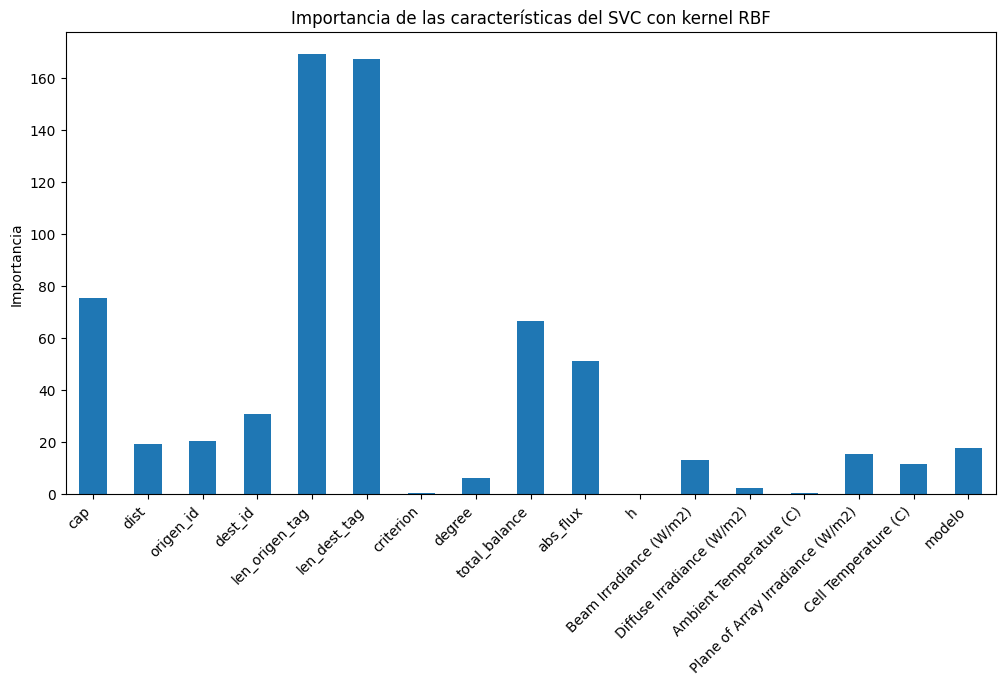
\includegraphics[width=1\textwidth]{img/desarrollo/svm/importance3.png}
    \caption{Puntuación de características del \acrshort{svm} mediante los atributos \textit{support\_vectors\_} y \textit{dual\_coef\_}}
    \label{fig:imp3}
\end{figure}

\pagebreak

Por otro lado, al igual que se ha expuesto para el \gls{rf} (ver Sección \ref{sec:rf1}), se incluye el análisis a partir del método de la permutación (\textit{permutation\_importance}). En este caso, las longitudes de las etiquetas siguen siendo predominantes, pero las características que hacen referencia a la capacidad y al flujo total de energía resultante de \gls{den2ne} (\textit{abs\_flux}) también presentan valores de puntuaciones a considerar.

\begin{figure}[H]
    \centering
    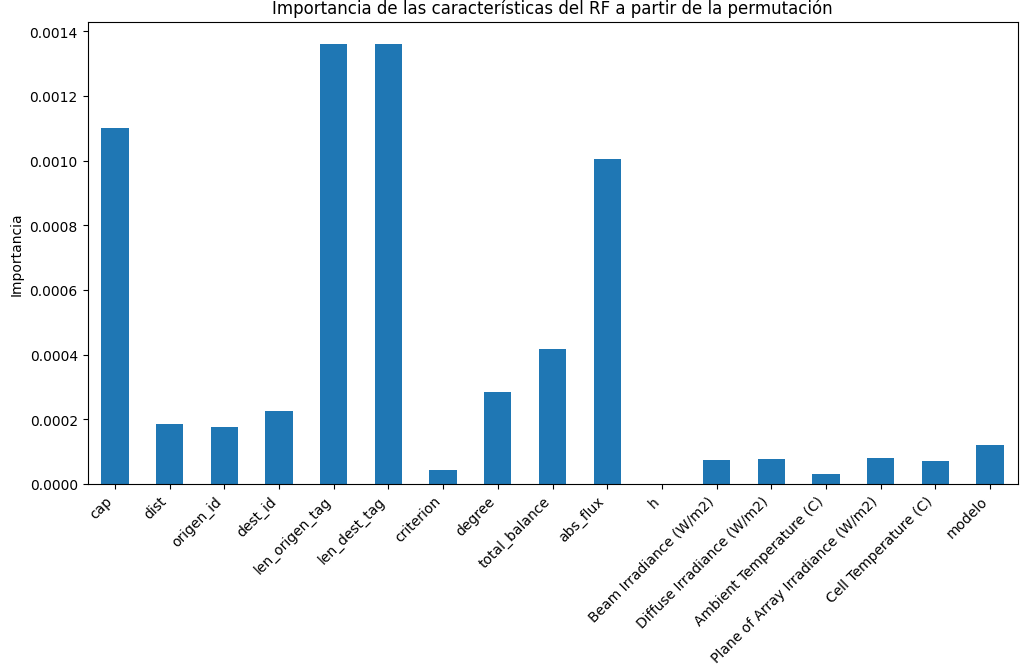
\includegraphics[width=1\textwidth]{img/desarrollo/svm/importance4.png}
    \caption{Puntuación de características del \acrshort{svm} mediante el método \textit{permutation\_importance}}
    \label{fig:imp4}
\end{figure}

\subsubsection{Optimización de hiperparámetros}
\label{sec:svm2}

Para modelar un \gls{svm} óptimo se centra el estudio en dos hiperparámetros: el tipo de kernel a aplicar y el parámetro de regularización \textit{C}. En el caso de \textit{gamma}, mencionada anteriormente, es indiferente su configuración, puesto que los datos del conjunto han sido previamente escalados (ver Sección \ref{sec:adicional}) y las dos opciones posibles de \textit{gamma} ('scale' o 'auto') únicamente se diferencian entre sí en la aplicación o no de la varianza de los datos en el cálculo del parámetro. 

\vspace{3mm}

\begin{lstlisting}[style=Python, caption={Cuadrícula de parámetros SVM}]
  param_grid = {
    'C': [0.25, 0.5, 0.75, 1], 
    'kernel': ['poly', 'rbf', 'sigmoid'] }
\end{lstlisting}

\vspace{3mm}

Después, se inicializa un objeto de la clase \textit{GridSearchCV()} y se configura de la misma forma que se detallaba en la Sección \ref{rf2} para el \gls{rf}. No obstante, teniendo en cuenta la gran duración del entrenamiento del modelo \gls{svm} en el paso anterior (ver Sección \ref{sec:svm1}), se debe cuantificar primero cuánto tiempo supone ejecutar todas las combinaciones de hiperaparámetros definidas en el método \textit{Grid Search}. Este cálculo se realiza en función de los pliegues configurados (\textit{cv=5}) y del número de procesadores, por lo que se estima el tiempo total de búsqueda de la combinación óptima en 349,4 horas.

\vspace{3mm}

La ejecución indica en los atributos \textit{best\_score\_} y \textit{best\_params\_} que el caso óptimo es un \gls{svm} basado en kernel radial o gaussiano (\gls{rbf}) con un parámetro de regularización \textit{C} igual a la unidad, con el que se alcanza una precisión del 97,78\%. No obstante, se debe llevar a cabo un análisis más detallado de los resultados de rendimiento de las combinaciones probadas a partir del atributo \textit{cv\_results\_}. Este diccionario aporta los valores promedio de precisión obtenida (\textit{mean\_test\_score}) como se muestra en la Tabla \ref{tab:svmgs}. Se pueden destacar variaciones en la precisión al aplicar los distintos tipos de kernel al clasificador, siendo el kernel sigmoide el que peores resultados proporciona. Sin embargo, el empleo de diferentes parámetros de regularización \textit{C} no implica grandes cambios en la precisión y, en el caso del kernel polinomial, es indiferente y se obtienen siempre los mismos valores. 

\vspace{3mm}

De la misma forma, se extrae también de \textit{cv\_results\_} el tiempo de entrenamiento (\textit{mean\_fit\_time}) que se ha dedicado para probar cada una de las combinaciones. Como se puede ver en la Tabla \ref{tab:svmgs2}, ahora el valor que toma el parámetro de regularización \textit{C} sí que incide de forma notable en los valores y aumenta de forma proporcional en el caso del kernel polinomial. Por ello, se puede expresar que si se desea emplear este tipo de kernel no sería adecuado configurar un parámetro de regularización alto, ya que el rendimiento empeora. 

\vspace{3mm}

\begin{table}[H]
  \centering
  \begin{subtable}{0.45\linewidth}
    \centering
    \begin{tabular}{|>{\columncolor[HTML]{EFEFEF}}c |c|c|c|}
      \hline
      \textit{\begin{tabular}[c]{@{}c@{}}Kernel /\\C\end{tabular}} & \cellcolor[HTML]{EFEFEF}\textit{poly} & \cellcolor[HTML]{EFEFEF}\textit{rbf} & \cellcolor[HTML]{EFEFEF}\textit{sigmoid}\\ \hline
      0,25 & 97,65 & 97,66 & 95,96 \\ \hline
      0,5 & 97,65 & 97,71 & 95,94 \\ \hline
      0,75 & 97,65 & 97,75 & 95,82 \\ \hline
      1 & 97,65 & 97,78 & 95,81 \\ \hline
    \end{tabular}
    \caption{Precisión (\%) (\textit{mean\_test\_score})}
    \label{tab:svmgs}
  \end{subtable}
  \hfill
  \begin{subtable}{0.45\linewidth}
    \centering
    \begin{tabular}{|>{\columncolor[HTML]{EFEFEF}}c |c|c|c|}
      \hline
      \textit{\begin{tabular}[c]{@{}c@{}}Kernel /\\C\end{tabular}} & \cellcolor[HTML]{EFEFEF}\textit{poly} & \cellcolor[HTML]{EFEFEF}\textit{rbf} & \cellcolor[HTML]{EFEFEF}\textit{sigmoid}\\ \hline
      0,25 & 21030 & 13876 & 14659 \\ \hline
      0,5 & 28807 & 10277 & 18695 \\ \hline
      0,75 & 42183 & 9328 & 12235 \\ \hline
      1 & 47460 & 9446 & 12869 \\ \hline
    \end{tabular}
    \caption{Tiempo (s) (\textit{mean\_fit\_time})}
    \label{tab:svmgs2}
  \end{subtable}
  \caption{Resultados extraídos del atributo \textit{cv\_results\_} del \acrshort{svm}}
  \label{tab:svmgs_combined}
\end{table}

\pagebreak

Sin embargo, mediante el análisis de los tiempos se confirma que la opción más adecuada a emplear es el caso óptimo descrito a priori por el atributo \textit{best\_params\_}, ya que proporciona un tiempo de entrenamiento relativamente bajo respecto al resto de combinaciones.

\subsubsection{Selección de características}
\label{sec:svm3}

Para el modelo de \gls{svm}, se procede a aplicar las mismas tres técnicas de reducción de la dimensionalidad del conjunto de datos que se utilizaron en el \gls{rf} (ver Sección \ref{sec:rf3}): \gls{rfecv}, \textit{kbest} y \gls{pca}. Sin embargo, en el caso de la primera, referente a la eliminación recursiva mediante validación cruzada, se encuentra con la problemática de que la clase del clasificador, \textit{SVC()}, no dispone de los atributos necesarios para su implementación (coef\_,  feature\_importances\_). Por ello, se tiene que descartar su uso y seguir con la aplicación del resto de técnicas.

\vspace{3mm}

En cuanto a la Selección Invariante de Características o \textit{kbest}, se mantiene la operativa realizada para el modelo de \gls{rf}. Como se comentaba en la Sección \ref{sec:rf3}, el número de características a seleccionar venía dado por la necesidad de realizar múltiples pruebas para encontrar el número óptimo que proporcionara la mayor precisión al modelo. Por ello, para simplificar este proceso, se aplicaban, dos valores de \textit{k} (\textit{k=5} y \textit{k=8}), siendo el segundo el dado como resultado de la técnica \gls{rfecv}. En este caso, como esta no se puede implementar, se toma la decisión de escoger los mismos valores que se configuraron en el modelo de \gls{rf}.

\vspace{3mm}

De la misma forma, en el caso del \gls{pca}, se repite el proceso descrito en la Sección \ref{sec:rf3}, aplicando la técnica para reducir las dimensiones del conjunto de datos a n=2 y n=4 componentes. 

\subsubsection{Ejecución del modelo y evaluación de resultados}
\label{sec:svm4}

Tras desarrollar el proceso de optimización de hiperparámetros del clasificador, se procede a evaluar el rendimiento del modelo \gls{svm} utilizando las diferentes técnicas de reducción de las dimensiones del conjunto de datos. Sin embargo, es importante volver a recalcar, antes de analizar los resultados, el significativo coste computacional y tiempo asociado con el entrenamiento del clasificador. En este caso, se ejecutan 5 pruebas aplicando en cada una el método de la matriz de confusión y del \textit{K-Fold Cross Validation}, lo que resulta en una duración total de 325 horas."

\vspace{3mm}

Para analizar los resultados de evaluación a partir de la matriz de confusión se proporciona la Tabla \ref{tab:svmcm}. Observando la misma, se puede destacar a simple vista que en los dos casos de aplicación del \gls{pca} se obtienen valores indefinidos en las métricas de \textit{Precision} y \textit{F1 Score}. Esto se debe a que el modelo de \gls{svm} no funciona correctamente y, por tanto, no logra realizar ninguna predicción de instancias positivas. Es por ello que, aunque se obtiene un valor de precisión global (\textit{Accuracy}) bueno, no es realmente eficiente. Respecto a esta métrica, si se visualizan las demás opciones, se obtienen también valores en torno al 97\%. En el caso de la precisión de detección de las instancias positivas (\textit{Precision}), la opción más favorable es la ejecución del modelo de \gls{svm} sin emplear ninguna técnica de reducción de dimensiones (89,32\%). En otros términos, al aplicar \textit{kbest} al conjunto de datos, se reduce la eficiencia cuanto menor es el número de características \textit{k} configurado (65,25\%).

\vspace{3mm}

Por otro lado, la métrica \textit{Recall} presenta en todas las opciones valores  bajos. Al referirse a la sensibilidad del modelo o, en otros términos, a la proporción de las instancias positivas que se identifican correctamente, el coste de predicción de errores se vuelve alto de forma general para el modelo. Con estos valores y los dados por \textit{F1 Score}, se puede expresar de una forma concluyente que el \gls{svm} no es lo suficientemente eficiente para detectar las instancias positivas. 

\vspace{3mm}

\begin{table}[H]
  \centering
  \begin{tabular}{|c|c|c|c|c|c|c|c|c|}
  \hline
  \rowcolor[HTML]{EFEFEF} 
  \textit{\begin{tabular}[c]{@{}c@{}}Matriz\\ de confusión\end{tabular}} & \cellcolor[HTML]{EFEFEF}\textit{TN} & \textit{FP} & \textit{FN} & \textit{TP} & \textit{Accuracy} & \textit{Precision} & \textit{Recall} & \textit{F1 Score} \\ \hline
  \cellcolor[HTML]{EFEFEF}\textit{Sin aplicar} & 377009 & 76 & 8489 & 634 & 97,23 & 89,32 & 6,95 & 12,83 \\ \hline
  \cellcolor[HTML]{EFEFEF}\textit{kbest (n=5)} & 376487 & 598 & 8002 & 1121 & 97,11 & 65,25 & 12,29 & 20,73 \\ \hline
  \cellcolor[HTML]{EFEFEF}\textit{kbest (n=8)} & 376742 & 343 & 8274 & 849 & 97,05 & 71,19 & 9,30 & 16,46 \\ \hline
  \cellcolor[HTML]{EFEFEF}\textit{PCA (n=2)} & 377085 & 0 & 9123 & 0 & 97,61 & - & 0 & - \\ \hline
  \cellcolor[HTML]{EFEFEF}\textit{PCA (n=4)} & 377085 & 0 & 9123 & 0 & 97,61 & - & 0 & - \\ \hline
  \end{tabular}
  \caption{Resultados de aplicación de la matriz de confusión al \gls{svm}}
  \label{tab:svmcm}
\end{table}

\vspace{3mm}

En cuanto a los resultados de aplicación del método \textit{K-Fold Cross Validation}, se puede que comprobar en la Tabla \ref{tab:svmk} que se obtienen valores de precisión parecidos a los dados anteriormente. En este caso, con mínimas diferencias, se presenta como mejor opción la aplicación de la técnica \textit{kbest} con 5 características con un 97,8\%.

\vspace{3mm}

Por tanto, tras completar el proceso de evaluación del modelo mediante ambos métodos, se puede expresar que se perciben generalmente mejores resultados para el \gls{rf} que para el \gls{svm}. Es decir, aunque los resultados de aplicar \textit{K-Fold Cross Validation} en ambos modelos no proporcionan precisiones significativamente diferentes entre sí (ver Tablas \ref{tab:rfk} y \ref{tab:svmk}), si se comparan las métricas calculadas a partir de las matrices confusión (ver Tablas \ref{tab:rfcm} y \ref{tab:svmcm}), el rendimiento que aporta el \gls{rf} es mucho mayor.

\vspace{3mm}

\begin{table}[H]
  \centering
  \begin{tabular}{|c|c|c|c|c|c|c|c|c|}
  \hline
  \rowcolor[HTML]{EFEFEF} 
  \textit{\begin{tabular}[c]{@{}c@{}}K-Fold\\ Cross Validation\end{tabular}} & \cellcolor[HTML]{EFEFEF}\textit{Accuracy(\%)} & \textit{Standard Deviation (\%)} \\ \hline
  \cellcolor[HTML]{EFEFEF}\textit{Sin aplicar} & 97,79 & 0,01 \\ \hline
  \cellcolor[HTML]{EFEFEF}\textit{kbest (n=5)} & 97,80 & 0,01 \\ \hline
  \cellcolor[HTML]{EFEFEF}\textit{kbest (n=8)} & 97,79 & 0,01 \\ \hline
  \cellcolor[HTML]{EFEFEF}\textit{PCA (n=2)} & 97,76 & 0,00 \\ \hline
  \cellcolor[HTML]{EFEFEF}\textit{PCA (n=4)} & 97,76 & 0,00 \\ \hline
  \end{tabular}
  \caption{Resultados de aplicación del \textit{K-Fold Cross Validation} al \gls{svm}}
  \label{tab:svmk}
\end{table}

